\chapter{\deisa: \dask-Enabled In Situ Analytics}



\epigraph{\textit{If I have seen further, it is by standing on the shoulders of Giants.}} {Issac Newton}



\section{introduction}

\section{The Bridging Model between BSP and Distributed Task-Based Paradigms}\label{sec:btp}

\subsection{Motivation}\label{sec:btp:motivation}
As already mentioned in the previous chapters, the in situ paradigm is a brilliant alternative to the post hoc. However, it becomes less relevant due to its setup complexity, which is due to the incompatibility of the MPI programming model with data analytics algorithms. To be able to explore the in situ paradigm with reduced complexity, we have mainly two possibilities: build both the simulation and the in situ tool with a higher-level programming model that makes the analytics easier to design or keep the simulation built on MPI and propose a bridging model between MPI and another programming model which is more adapted for analytics.

The first possibility is not a relevant solution because it means that we will need to write simulation codes in another programming model, likely higher-level and slower, which is not a good idea for the reasons we mentioned in section\ref{BSP} about the success of MPI and BSP in general. 
The second possibility is more interesting as it will keep the BSP programming model for the simulations, choose a more adapted model for analytics and propose a bridging model to couple them. 
In this work, we have opted for the second solution and chosen the task-based programming model for the in situ analytics for the easiness it brings as well as the variety of tools that are already available and usable for different data processing.   

% I moved this from chapter01:theory:discussion 

The BSP and the Task-based paradigms differ not only in terms of abstraction levels, development effort, and performance but also in defining key concepts such as parallelism and the data and how they are managed.

First of all, the type of parallelism in BSP, let us take MPI as an example; the application is represented as a set of $P$ processes, each with its local memory and buffers. The parallelism in the task-based model is expressed in terms of tasks and dependencies. While the user is responsible for creating the processes and their management in MPI, a runtime ensures that job in task-based models. We talk about explicit parallelism in MPI and implicit one in the task-based programming model. 
Secondly, the data semantics and representation in those models are different too. As defined in MPI, the data are buffers that keep the same name during execution and whose values are updated as the simulation progresses. Hence the data in MPI can be defined as the value of a given variable at a specific moment.
In task-based models, data are immutable and defined either as an input or an output of a given task. While the timestep is important to identify needed data in MPI, it does not have a similar signification in a task-based model. 
The third big difference is related to the view we may have about an application in both cases. While a task graph describes all the tasks that will be run in a task-based model, it is complex and sometimes impossible for BSP applications to have such a view from the beginning. And this makes the coupling more challenging, as we do not have any a priori idea about what will be executed at runtime, the data that will be generated, and when they are shared.

Those conceptual differences make coupling codes coming from the two paradigms challenging. To reduce this complexity and take advantage of both paradigms, we propose the Bulk Task Parallel paradigm that brings together the BSP and the task-based paradigms. 


\subsection{The Bulk Task Parallel bridging model}\label{sec:btp:btpmdel}

We define the Bulk Task Parallel(BTP), the new bridging model that couples BSP with distributed task-based programs. In the frame of this work, we only consider a producer/consumer scheme where the producer is parallelized following the BSP model and the consumer is in a task-based model.  The BTP is built on top of basic concepts, namely: BTP tasks (section~\ref{btptask}), exchange points (section~\ref{EP}) and delivery facilities (section~\ref{DF}).  

Let an \textbf{\textit{Actor}} be the union of a code and all its necessary resources: processing and memory units.   
For instance, let $A_{BSP}^{R_{1}}$ be an \textit{Actor} where $A$ is a BSP implementation of a problem $P_{1}$, and $R1$ is the needed resources for $P_{1}$ to be run, and let $B_{Task}^{R_{2}}$ be an \textit{Actor} where $B$ is a Task-based implementation of a problem $P_{2}$, and $R_{2}$ is the needed resources.

\subsubsection{BTP Tasks}\label{btptask}
Let $S_{BSP}^{R_{s}}$ be an iterative code (a simulation code for instance). Let \textbf{C} be a computation and let \textbf{Cmn} be a communication performed internally to the \textit{Actor} (MPI communication for instance). The smallest \textit{Task} that can be defined in a BSP model is the union of all computations \textbf{C} that are delimited by two communications \textbf{Cmn}. 

A \textit{BTP task} can be seen as a \textit{Task} where we distinguish internal and external communications. It is a set of computations \textbf{C} and internal communications \textbf{Cmn}, delimited by two \textit{Exchange Point} (a possible external communication). In \textit{Task-based} model we distinguish the internal (to the \textit{Actor}) input/output data from the external ones (where the source/destination) is another \textit{Actor}. Hence, a \textit{BTP task} is a subgraph that is delimited by two external communications done through \textit{Exchange Points}.


\begin{figure}[tb]\centering
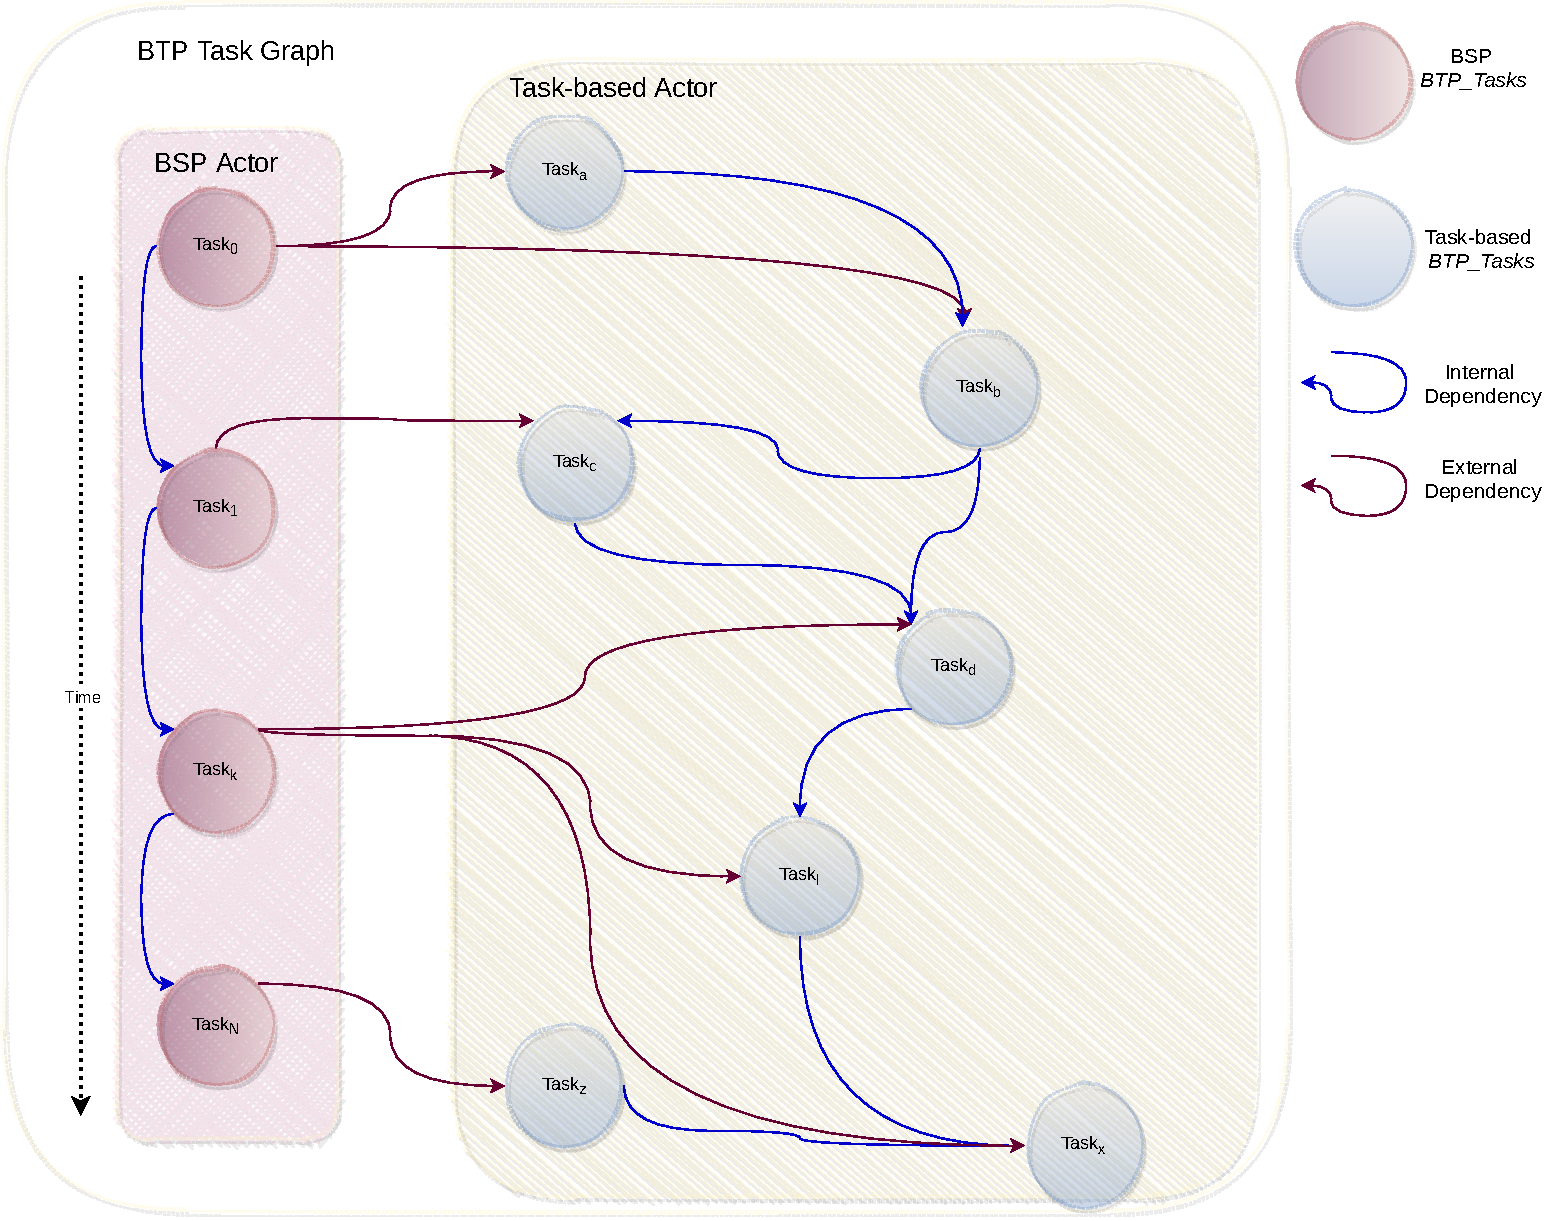
\includegraphics[width=0.75\columnwidth]{figures/BTPTaskGraph.pdf}
\caption{BTP task graph}
\label{figWUG}
\end{figure}

\subsubsection{Exchange Point}\label{EP}

An \textit{Exchange Point} (EP) can be defined as an entry point to BTP model. An \textit{Actor} shares through it an internal data with other \textit{Actors}. The main motivation to introduce \textit{Exchange points} is to keep a good separation of concerns. It provides a clean way to couple \textit{Actors}. For instance \textit{Actor A} can through its \textit{EPs} expose an array \textit{A} for external use. \textit{Actor B} does not need to know how \textit{Actor A} computes this array, and \textit{Actor A} needs to know neither which data \textit{Actor B} needs nor how it will use it.

The only way to get information about data an \textit{Actor} generates is by establishing a connection with it through a \textit{Delivery Facility} and checking available data (the data that \textit{A} wants to share) in the \textit{Exchange points}.

\subsubsection{Delivery Facility}\label{DF}

In addition of ensuring the establishment of connections between \textit{Actors}, the \textit{Delivery Facility} (DF) ensures a global identification and redistribution of data between \textit{Actors}. Hence,  it can be split to 3 main components : a \textit{Connection Facility} a \textit{Data Identification Component}, a \textit{Data Redistribution Component}.
\begin{itemize}
   \item \textit{Connection Facility} (CF): it establishes connections and communication with remote actors.
   \item \textit{Data Identification Component} (DIC): is responsible for the identification of a piece of data internally in an \textit{Actor} and translate its identifier to a global ID understandable in other \textit{Actors}. The step of identification is essential due to the different ways data is defined in the two paradigms. 
   
   \item \textit{Data Redistribution Component} (DRC): implements a data redistribution scheme. It is aware of the number of the resources $R$ (processes or workers) in the \textit{Actor} $Consumer_{Paradigm}^{R}$ and maps each data to a set of resources.
\end{itemize}

\subsection{Porting a BSP code to BTP semantic}\label{sec:btp:porting}

\begin{figure*}[tb]
\centerline{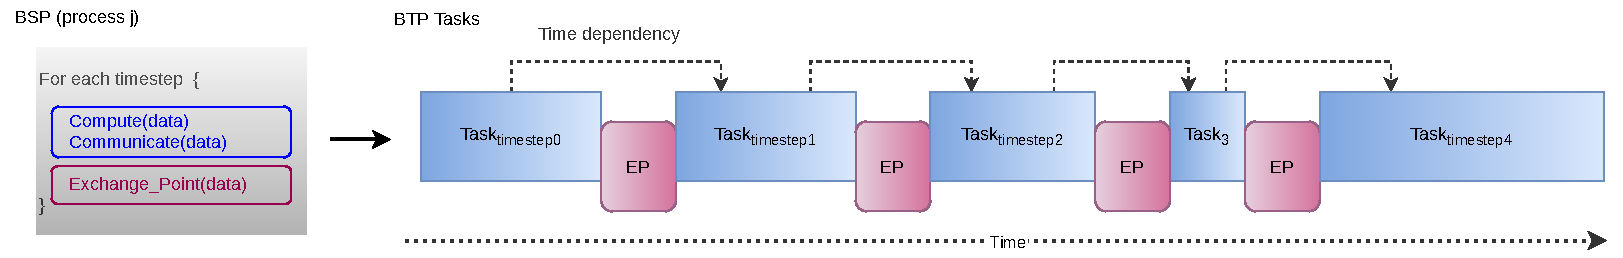
\includegraphics[width=\textwidth]{figures/unrolled.pdf}}
\caption{Example of BTP representation for an iterative BSP code}
\label{figunroll}
\end{figure*}

We suppose that the BSP \textit{Actor} is an iterative code parallelized in MPI. The code does not need to be rewritten to be designed in the BTP semantic. What needs to be done is only to tag the data we want to share externally and specify when this will be done. Concretely, calls to \texttt{Exchange\_point} are added in the simulation code to make data available for external use. By definition, a \textit{BTP task}, in BSP words, is a set of computations and internal communications that are delimited by two \textit{EPs}; concretely, it is all the code that is delimited by two calls of \texttt{Exchange\_point}. The call to \texttt{Exchange\_point} that is added at the end of each iteration in the loop in fig.~\ref{figunroll} is enough to construct a list of \textit{BTP tasks}, one per each time step. It is similar to an unrolled loop over time.


\subsection{Full Producer Consumer Example}\label{sec:btp:FullPCExample}

 
\begin{figure}[tb]\centering
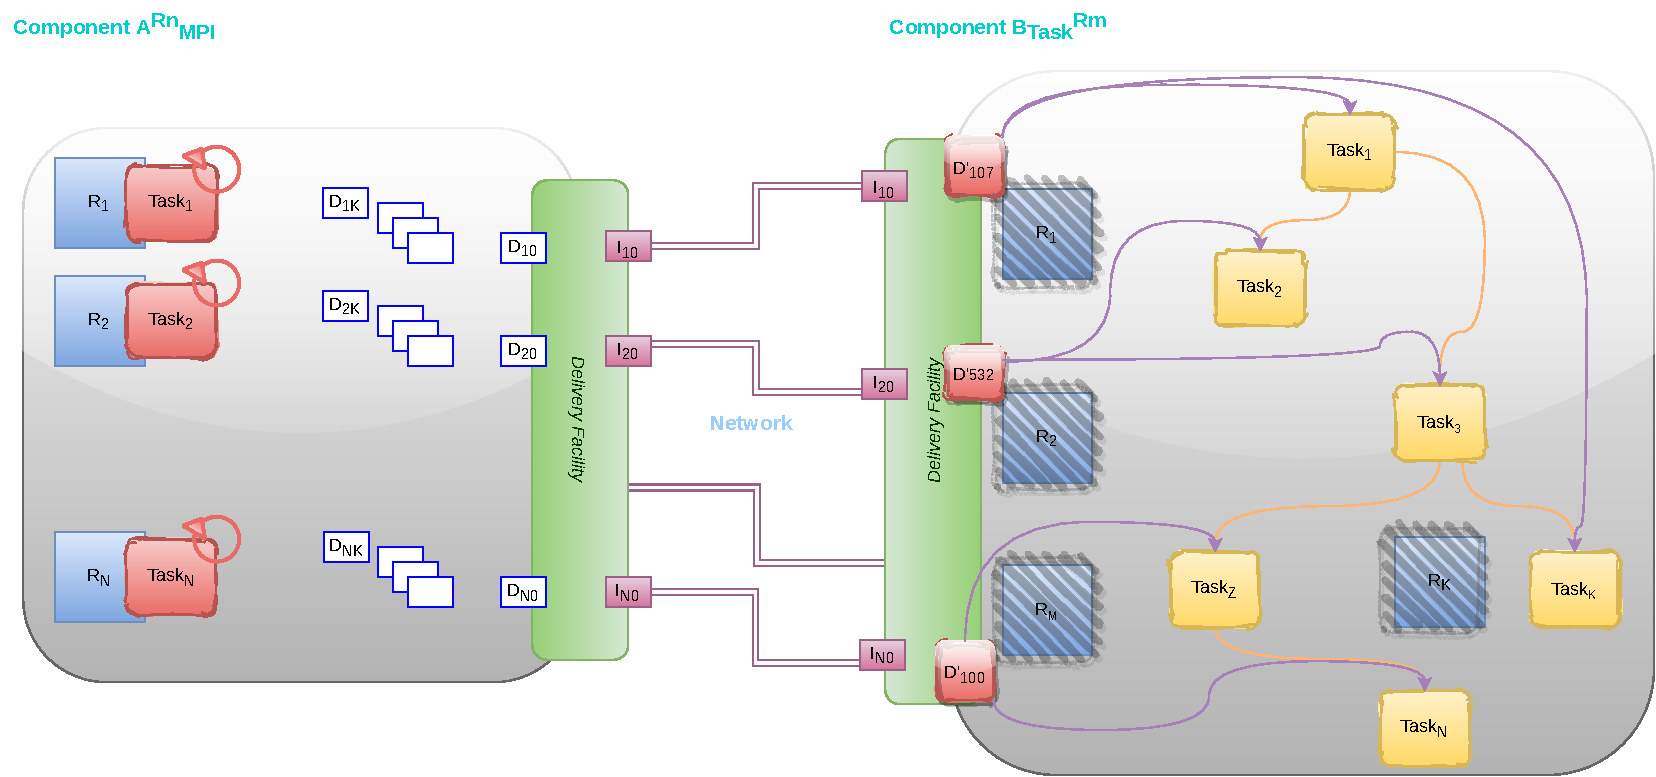
\includegraphics[width=\columnwidth]{figures/BTP.pdf}
\caption{producer consumer example}
\label{figBTP}
\end{figure}

Figure~\ref{figBTP} shows an example coupling $A_{BSP}^{R_{n}}$ and $B_{Task}^{R_{m}}$ where \textit{Actor A} is a producer and \textit{Actor B} is a consumer. The BSP \textit{Actor} has $R_{n}$ resources. Each $Task_k$ is scheduled explicitly to a set of resources $R_{k}$. In scientific applications, we usually have an iterative code. Each \textit{Task} generates a block of data at a given timestep $t$ (only one \textit{Task} is shown in the figure, with a loop mark). Those blocks of the data (small blue boxes $D_{i,j}$) are shared through the \textit{Exchange points} (not represented in the figure) and sent to the \textit{Delivery Facility}.
\textit{Actor B} is the consumer of the data. It is a task-based \textit{Actor}, has $R_{m}$ resources that are managed implicitly by a runtime (blue boxes with grey hachures). A task graph is represented as a BTP \textit{Task} graph (yellow graph), with dependencies on external inputs. Those inputs (in red) are data with new keys (IDs) that are easily recognizable, thus usable in \textit{Actor B}.  

The data are sent through the network between \textit{Actors}. The \textit{DFs} ensure the connection to a distant \textit{Actor}, the identification and redistribution of data between \textit{Actors}. 
In this figure, the data identification is made in two steps from each side. The small blue boxes $D_{i,j}$ are identified by three elements: $D$ is the name of the data, $i$ is the MPI rank (for instance or the position of this block of data in the global distribution), and the $j$ corresponds to the timestep. These keys can be considered as local to the \textit{Actor A}. 
In the same Actor, a new key has been created $I_{l,m}$. It is a global key recognizable in the \textit{DF} of \textit{Actor B}. In the \textit{Actor B}, those keys are translated to new keys internally understandable $D'_{k}$. 
This identification and translation process can be done in fewer steps. For example, if $I_{l,m}$ is recognizable by \textit{Actor B}, then there is no need for further translation at reception.

\section{BTP Implementation}\label{sec:btpimplementation}
Several choices have been made regarding the implementation of the BTP paradigm. We have focused on three main goals: performance and separation of concerns on the simulation side and productivity on the analytics side. All our choices have been guided by those goals to propose a solution that responds the most to the main motivation of this thesis, namely: bringing together the performance of in situ and the productivity we were used to in post hoc workflows, for that we have opted to use focus on the MPI implementation of BSP to parallelize simulation codes, \pdi data interface to handle data and implement the \textit{Delivery facily} engine, \dask distributed as a task-based framework to introduce a distributed pythonic environment in in situ paradigm. 
We have chosen MPI for its success and popularity in the HPC community; all legacy and new production codes are parallelized in MPI+X. We will focus here on justifying our choice regarding \pdi and \dask.

As already presented in section~\ref{sec:pdi}, \pdi is a lightweight data handling library that keeps an outstanding separation of concerns. With its declarative API, it enables sharing of simulation data for external use without any copy, thus its performance. In addition, it allows changing the data handling approach in the external configuration file without recompiling the simulation code. \pdi is already used in several production codes such as Gysela\cite{bigot:hal-01050322-gysela, latu:hal-01834323-gysela, latu:hal-01719208-gysela} to handle their IOs with \texttt{decl'hdf5} or for check-pointing using \texttt{FTI} plugin.      
In this work, we have chosen to use \pdi to extract simulation data as an \textit{Exchange Point}, and implemented the \textit{Data Facility} through a new \pdi plugin named \deisa. In addition to the advantages listed above, \pdi allows switching between different plugins easily, thus switching between in situ and post hoc modes; such an advantage is crucial to support heterogeneous workflows to be able to keep analytics results along with brute data in case further analytics are needed. 

One of the main issues in the in situ approach is its setup complexity. In this work, we introduce an outstanding ease-of-use in in situ workflows which is comparable to post hoc ones and bring the zen of python to the HPC community, all in one through \dask distributed. Among other data analytics frameworks, we have opted for \dask (to be our distributed task-based framework) because it offers distributed APIs for well-known python libraries such as \texttt{numpy}, \texttt{pandas} and \texttt{scikit-learn}. A post hoc sequential python code is easily ported to in situ distributed \dask code thanks to BTP paradigm.     




\subsection{Data Model}\label{sec:btpImp:datamodel}
Data is one of the core concepts of our work; its definition, identification, representation, and communication are as important as its processing. To smooth  differences between BSP and task-based model(mentioned in section~\ref{sec:btp:motivation}), the \textit{Delivery Facilities} from both sides, being aware of the definition of data, adds a layer to make it understandable in the other model. Data being a value of a given variable at a given timestep, in MPI, needs an MPI communicator as well as a rank to be identified in the global distribution of the array generated by a simulation.    

\subsubsection{Data Definition}\label{sec:datamodel:datadef}
from ptr - pdi pybind -  pycall - numpy - dask

\subsubsection{Data Identification}\label{sec:datamodel:dataid}
%metadata
what and how and why 
keys we get from a scatter, the size and position are sent 
used for dask array creation 
\subsubsection{Data Representation}\label{sec:datamodel:datarepresent}
%Deisa virtual arrays
from the simulation side as a mirror of the dask array that we create in the client side.

\subsection{Data and Control Communication}
\subsubsection{Control}
All control goes through the scheduler, but we can optimize it through mpi as future work 
\paragraph{Queues} 

\paragraph{Variables}
when several clients need the same data 

\subsubsection{Data communication}
\paragraph{Deisa Bridge}
deisa plugin/ pycall
light client + far heartbeat 
limit 512 ..

\subsection{Data semantic}
in /out  data in a task vs same var and different values per time step in mpi

\subsection{Time-independent task submission}

\subsection{Steering}
limit generated data, but steering in the other sense can be done easily  
\subsubsection{Queues}
\subsubsection{Contracts}
\subsection{Dynamic scheduling}
triggers I have to do that 

\amal{pas implementation je ne sais pas trop }
\subsection{Implementation}

\cite{deisa}

\subsubsection{Architecture}
\begin{figure}[tb]\centering
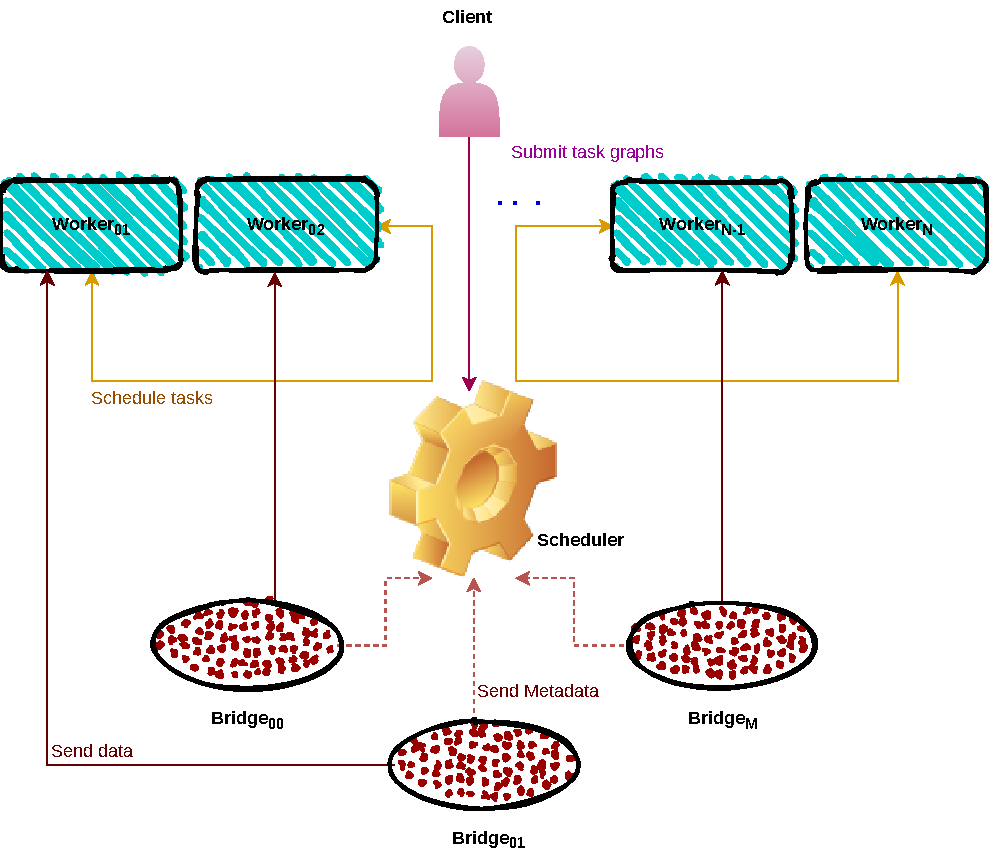
\includegraphics{figures/ArchiectureDeisa.pdf}
\caption{\deisa}
\label{figdeida}
\end{figure}

\begin{figure}[tb]\centering
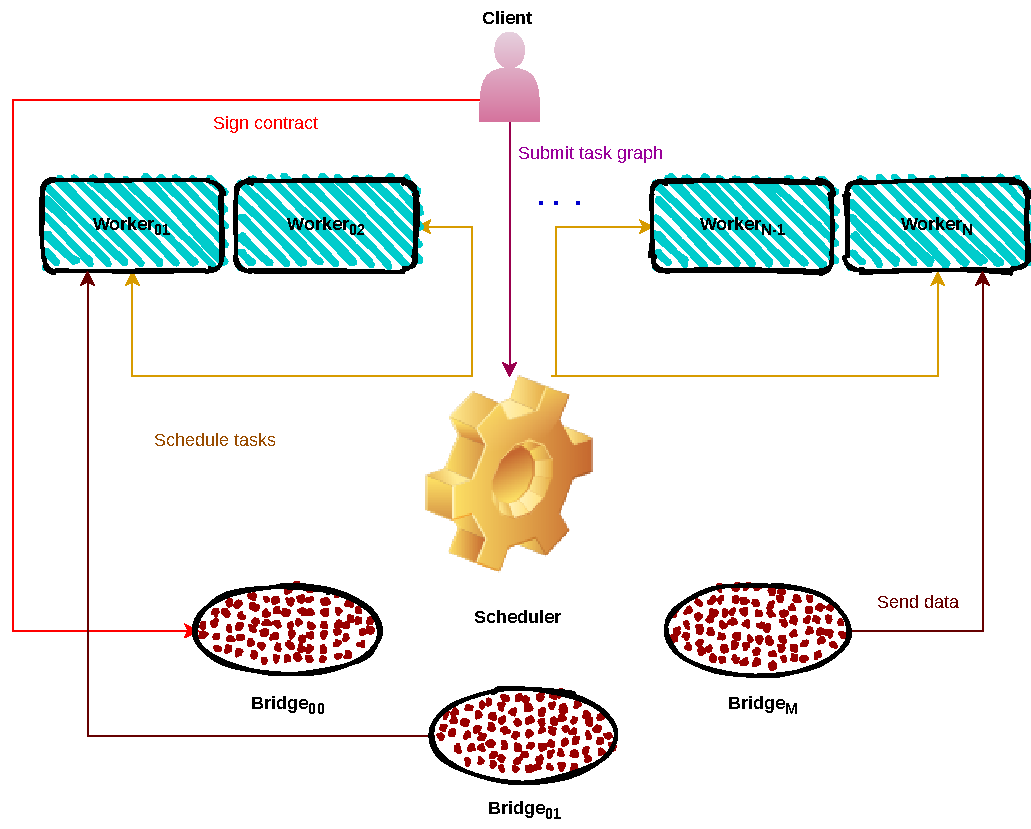
\includegraphics{figures/ArchiectureDeisaV2.pdf}
\caption{\deisa v2}
\label{figdeidav2}
\end{figure}
\subsubsection{API}
just the last one 
\subsubsection{Instrumentation}
\begin{lstlisting}[float, label=ymldata, language=yaml, caption=Data description in \pdi \deisa YAML file]
types: #[...] including config_t description
metadata: {step: int, cfg: config_t, rank: int} |\label{ymldata:metadata}|
data: 
plugins:
  mpi: # get MPI rand and size
  deisa:
    scheduler_info: scheduler.json
    init_on: init 
    time_step: $step 
    deisa_arrays: # Deisa Virtual arrays
      G_temp: # Field name
        type: array
        subtype: double
        size:
          -timedim 
          -'$cfg.loc[0] * ($rank % $cfg.proc[0])'
          -'$cfg.loc[1] * ($rank / $cfg.proc[0])'
        subsize: [1, '$cfg.loc[0]', '$cfg.loc[1]'] # chunk size
        start:  # chunk start
          -$step
          -'$cfg.loc[0] * ($rank % $cfg.proc[0])'
          -'$cfg.loc[1] * ($rank / $cfg.proc[0])'
        +timedim: 0 # a tag for the time dimension
    map_in: # deisa array mapping
      temp: G_temp
        
\end{lstlisting}
\subsubsection{Evaluation}
\subsubsection{Limitations}

\section{Conclusion}